\subsection{Aktivitas}

Aktivitas pada \textit{software deployment} terdiri dari
\textit{release}, \textit{installation}, \textit{activation}, \textit{deactivation}, \textit{retire}, \textit{update}, \textit{reorganization}, serta \textit{redistribution}. Berikut merupakan penjelasan tentang tahapan tersebut serta visualisasinya yang dapat dilihat pada Gambar II.1.

\begin{enumerate}
  \item \textit{Release} adalah tahapan untuk mempersiapkan \textit{software} untuk didistribusikan
  \item \textit{Installation} adalah tahapan awal untuk melakukan \textit{integrasi} \textit{software} pada perangkat pengguna.
  \item \textit{Activation} adalah proses yang dilakukan ketika menyalakan \textit{software}.
  \item \textit{Deactivation} adalah proses untuk menghentikan \textit{software}.
  \item \textit{Deinstallation} adalah proses untuk menghilangkan seluruh bagian dari \textit{software} pada perangkat pengguna.
  \item \textit{Retire} adalah proses untuk menandakan bahwa \textit{software} sudah bersifat \textit{obsolete} dan tidak akan dilakukan \textit{maintanance} lagi.
  \item \textit{Update} adalah proses membuat versi terbaru dari \textit{software}.
\end{enumerate}

\begin{figure}[ht]
  \centering
  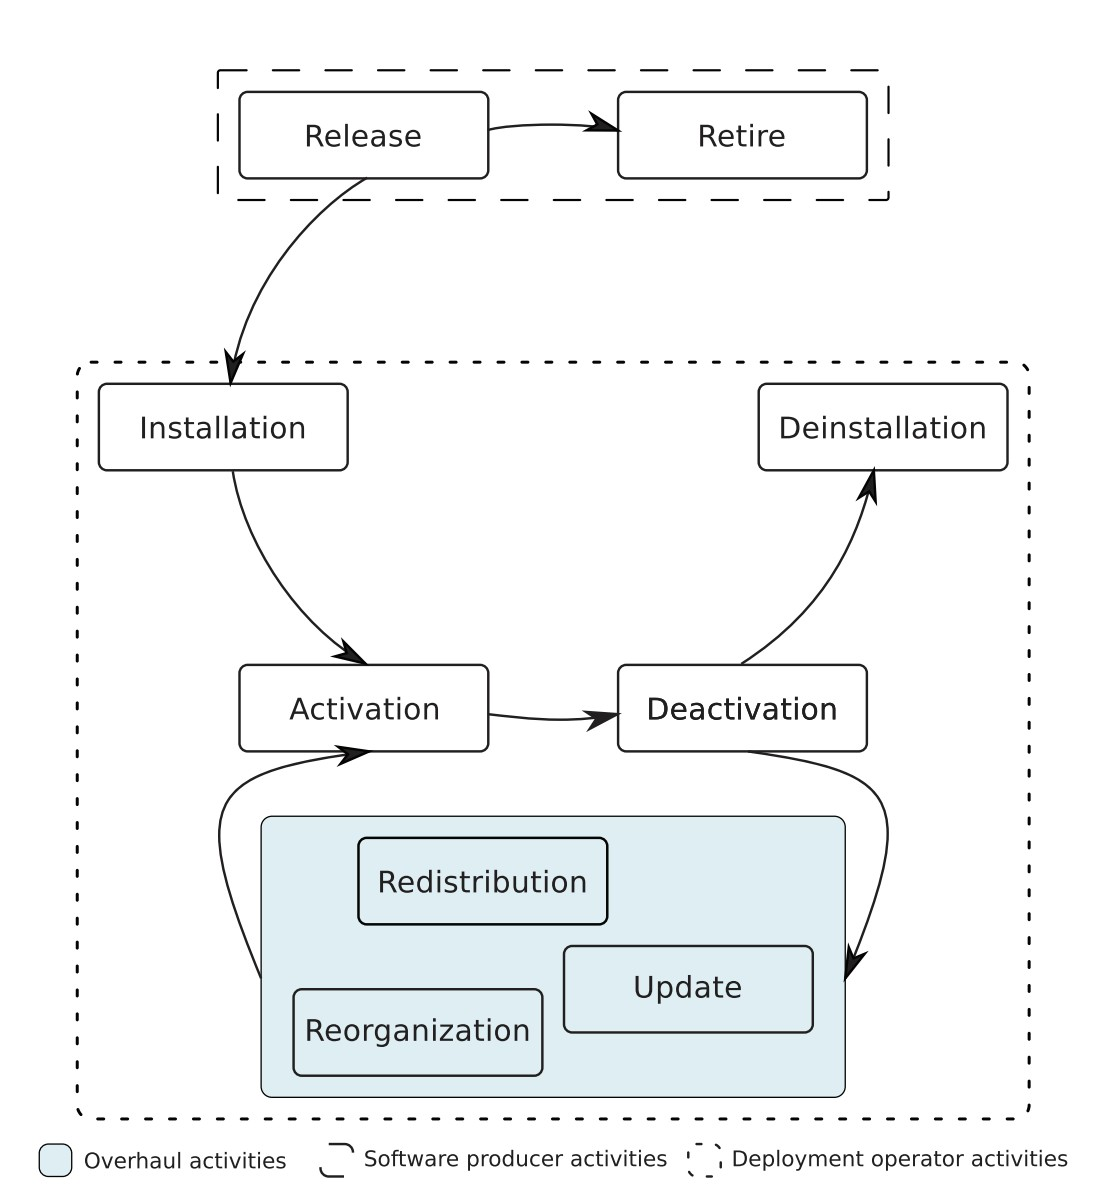
\includegraphics[width=0.8\textwidth]{resources/chapter-2/deployment-phase.jpg}
  \caption{\textit{Deployment Phase \parencite{ARCANGELI2015198}}}
  \label{fig:deployment-phase}
\end{figure}